%!Mode:: "TeX:UTF-8"
\documentclass[a4paper,11pt,UTF8]{ctexart}

\usepackage{indentfirst} %缩进
\usepackage{xeCJK}    %使用系统字体
\usepackage{fancyhdr} %自定义页眉页脚
\pagestyle{empty}                   %不设置页眉页脚
\usepackage{amsmath, amsthm, amssymb, amsfonts} %数学公式
\usepackage[a4paper,left=3cm,right=3cm,top=3cm,bottom=3cm]{geometry}
%\usepackage[tmargin=1in,bmargin=1in,lmargin=1.25in,rmargin=1.25in]{geometry}.
\usepackage{booktabs} %插入表格
\usepackage[section]{placeins} %避免浮动
\usepackage{listings} %插入代码
\usepackage{ctex}     %中文宏包
\usepackage[svgnames, table]{xcolor} %彩色表格
\usepackage{algorithm}          %伪代码
\usepackage{algorithmicx}
\usepackage{algpseudocode}
\usepackage{algorithm,algpseudocode,float}
\usepackage{lipsum}
\usepackage{enumitem}           %调整列举环境
\usepackage{url}
\usepackage{fontspec,xunicode}
\defaultfontfeatures{Mapping=tex-text} %如果没有它,会有一些 tex 特殊字符无法正常使用,比如连字符。

\usepackage{graphicx}
\graphicspath{{imgs/}}

%%%%%%%%%%%%%%%%%%%%%%%%%%%%%%%%%%%%%%%%%%%%%%%%%%%%%%%%%%%%%%%%
% 缩进及行间距
%%%%%%%%%%%%%%%%%%%%%%%%%%%%%%%%%%%%%%%%%%%%%%%%%%%%%%%%%%%%%%%%
\setlength{\parindent}{22pt} %重新定义缩进长度
\setlength{\baselineskip}{20pt}  %定义行间距
%\renewcommand{\baselinestretch}{1.1} %定义行间距

%%%%%%%%%%%%%%%%%%%%%%%%%%%%%%%%%%%%%%%%%%%%%%%%%%%%%%%%%%%%%%%%
% 列表设置
%%%%%%%%%%%%%%%%%%%%%%%%%%%%%%%%%%%%%%%%%%%%%%%%%%%%%%%%%%%%%%%%
\setenumerate{fullwidth,itemindent=\parindent,listparindent=\parindent,itemsep=0ex,partopsep=0pt,parsep=0ex}
\setenumerate[2]{label=\alph*),leftmargin=1.5em}  %二级item设置
\setitemize{itemindent=38pt,leftmargin=0pt,itemsep=-0.4ex,listparindent=26pt,partopsep=0pt,parsep=0.5ex,topsep=-0.25ex}
\setdescription{itemindent=38pt,leftmargin=0pt,itemsep=-0.4ex,listparindent=26pt,partopsep=0pt,parsep=0.5ex,topsep=-0.25ex}

%%%%%%%%%%%%%%%%%%%%%%%%%%%%%%%%%%%%%%%%%%%%%%%%%%%%%%%%%%%%%%%%
% 图的标题行间距设置
%%%%%%%%%%%%%%%%%%%%%%%%%%%%%%%%%%%%%%%%%%%%%%%%%%%%%%%%%%%%%%%%
\newcommand{\bottomcaption}{%
\setlength{\abovecaptionskip}{6pt}%
\setlength{\belowcaptionskip}{6pt}%
\caption}


%%%%%%%%%%%%%%%%%%%%%%%%%%%%%%%%%%%%%%%%%%%%%%%%%%%%%%%%%%%%%%%%
% 字体定义
%%%%%%%%%%%%%%%%%%%%%%%%%%%%%%%%%%%%%%%%%%%%%%%%%%%%%%%%%%%%%%%%
\setmainfont{Times New Roman}  %默认英文字体.serif是有衬线字体sans serif无衬线字体
\setmonofont{Consolas}
\setCJKmainfont[ItalicFont={楷体}, BoldFont={黑体}]{宋体}%衬线字体 缺省中文字体为
\setCJKsansfont{黑体}
\punctstyle{hangmobanjiao}
%-----------------------xeCJK下设置中文字体------------------------------%
\setCJKfamilyfont{song}{SimSun}                             %宋体 song
\newcommand{\song}{\CJKfamily{song}}
\setCJKfamilyfont{fs}{FangSong}                      %仿宋  fs
\newcommand{\fs}{\CJKfamily{fs}}
\setCJKfamilyfont{ktgb}{KaiTi}                      %楷体2312 ktgb
\newcommand{\ktgb}{\CJKfamily{ktgb}}
\setCJKfamilyfont{yh}{Microsoft YaHei}                    %微软雅黑 yh
\newcommand{\yh}{\CJKfamily{yh}}
\setCJKfamilyfont{hei}{SimHei}                              %黑体  hei
\newcommand{\hei}{\CJKfamily{hei}}
\setCJKfamilyfont{hwxk}{STXingkai}                                %华文行楷  hwxk
\newcommand{\hwxk}{\CJKfamily{hwxk}}
%------------------------------设置字体大小------------------------%
\newcommand{\shiyanbaogao}{\fontsize{36pt}{\baselineskip}\selectfont}
\newcommand{\chuhao}{\fontsize{42pt}{\baselineskip}\selectfont}     %初号
\newcommand{\xiaochuhao}{\fontsize{36pt}{\baselineskip}\selectfont} %小初号
\newcommand{\yihao}{\fontsize{28pt}{\baselineskip}\selectfont}      %一号
\newcommand{\erhao}{\fontsize{21pt}{\baselineskip}\selectfont}      %二号
\newcommand{\xiaoerhao}{\fontsize{18pt}{\baselineskip}\selectfont}  %小二号
\newcommand{\sanhao}{\fontsize{15.75pt}{\baselineskip}\selectfont}  %三号
\newcommand{\sihao}{\fontsize{14pt}{\baselineskip}\selectfont}       %四号
\newcommand{\xiaosihao}{\fontsize{12pt}{\baselineskip}\selectfont}  %小四号
\newcommand{\wuhao}{\fontsize{10.5pt}{\baselineskip}\selectfont}    %五号
\newcommand{\xiaowuhao}{\fontsize{9pt}{\baselineskip}\selectfont}   %小五号
\newcommand{\liuhao}{\fontsize{7.875pt}{\baselineskip}\selectfont}  %六号
\newcommand{\qihao}{\fontsize{5.25pt}{\baselineskip}\selectfont}    %七号

%%%%%%%%%%%%%%%%%%%%%%%%%%%%%%%%%%%%%%%%%%%%%%%%%%%%%%%%%%%%%%%%
% 图题字体大小相同
%%%%%%%%%%%%%%%%%%%%%%%%%%%%%%%%%%%%%%%%%%%%%%%%%%%%%%%%%%%%%%%%
\usepackage{caption}
\captionsetup{font={footnotesize}}   % footnotesize = 9pt
\captionsetup[lstlisting]{font={footnotesize}}

%%%%%%%%%%%%%%%%%%%%%%%%%%%%%%%%%%%%%%%%%%%%%%%%%%%%%%%%%%%%%%%%
% 重定义枚举编号为 1),2)...
%%%%%%%%%%%%%%%%%%%%%%%%%%%%%%%%%%%%%%%%%%%%%%%%%%%%%%%%%%%%%%%%
\renewcommand{\labelenumi}{\theenumi)}


%%%%%%%%%%%%%%%%%%%%%%%%%%%%%%%%%%%%%%%%%%%%%%%%%%%%%%%%%%%%%%%%
% 重定义section标题
%%%%%%%%%%%%%%%%%%%%%%%%%%%%%%%%%%%%%%%%%%%%%%%%%%%%%%%%%%%%%%%%
\CTEXsetup[format={\sihao\CJKfamily{zhhei}\zihao{4}},number={\chinese{section}},name={,、~},aftername={},indent={0pt},beforeskip={6pt},afterskip={6pt},format+={\flushleft}]{section}
\CTEXsetup[format={\Large\bfseries\CJKfamily{zhkai}\zihao{5}},name={(,)},number={\chinese{subsection}},aftername={},indent={22pt},beforeskip={14pt},afterskip={2pt}]{subsection}
\CTEXsetup[number={\chinese{section}},name={附录, ~~ }]{appendix}



%%%%%%%%%%%%%%%%%%%%%%%%%%%%%%%%%%%%%%%%%%%%%%%%%%%%%%%%%%%%%%%%
% 标题名称中文化
%%%%%%%%%%%%%%%%%%%%%%%%%%%%%%%%%%%%%%%%%%%%%%%%%%%%%%%%%%%%%%%%
\renewcommand\figurename{\hei 图}
\renewcommand\tablename{\hei 表}
\renewcommand\lstlistingname{\hei 代码}
\renewcommand{\algorithmicrequire}{\textbf{输入:}}
\renewcommand{\algorithmicensure}{\textbf{输出:}}
\newtheorem{define}{定义}

%%%%%%%%%%%%%%%%%%%%%%%%%%%%%%%%%%%%%%%%%%%%%%%%%%%%%%%%%%%%%%%%
% 代码设置
%%%%%%%%%%%%%%%%%%%%%%%%%%%%%%%%%%%%%%%%%%%%%%%%%%%%%%%%%%%%%%%%
\lstset{
 columns=fixed,
 numbers=left,                                        % 在左侧显示行号
 numberstyle=\tiny\color{gray},                       % 设定行号格式
 frame=single,                                        % 单线背景边框
 breaklines=true,                                     % 设定LaTeX对过长的代码行进行自动换行
 keywordstyle=\color[RGB]{40,40,255},                 % 设定关键字颜色
 numberstyle=\footnotesize\color{darkgray},
 commentstyle=\it\color[RGB]{0,96,96},                % 设置代码注释的格式
 stringstyle=\rmfamily\slshape\color[RGB]{128,0,0},   % 设置字符串格式
 showstringspaces=false,                              % 不显示字符串中的空格
 language=java,                                        % 设置语言
 basicstyle=\linespread{1.0}\xiaowuhao\ttfamily,                      % 字体字号
 %lineskip=10pt,
 %baselinestretch=1,
}

%%%%%%%%%%%%%%%%%%%%%%%%%%%%%%%%%%%%%%%%%%%%%%%%%%%%%%%%%%%%%%%%
% 伪代码分页
%%%%%%%%%%%%%%%%%%%%%%%%%%%%%%%%%%%%%%%%%%%%%%%%%%%%%%%%%%%%%%%%
\makeatletter
\renewcommand{\ALG@name}{算法}
\newenvironment{breakablealgorithm}
  {% \begin{breakablealgorithm}
   \begin{center}
     \refstepcounter{algorithm}% New algorithm
     \hrule height.8pt depth0pt \kern2pt% \@fs@pre for \@fs@ruled
     \renewcommand{\caption}[2][\relax]{% Make a new \caption
       {\raggedright\textbf{\ALG@name~\thealgorithm} ##2\par}%
       \ifx\relax##1\relax % #1 is \relax
         \addcontentsline{loa}{algorithm}{\protect\numberline{\thealgorithm}##2}%
       \else % #1 is not \relax
         \addcontentsline{loa}{algorithm}{\protect\numberline{\thealgorithm}##1}%
       \fi
       \kern2pt\hrule\kern2pt
     }
  }{% \end{breakablealgorithm}
     \kern2pt\hrule\relax% \@fs@post for \@fs@ruled
   \end{center}
  }
\makeatother



\begin{document}
\xiaosihao\song

\begin{titlepage}
\center{\yihao{\hwxk{武汉大学国家网络安全学院}}}
\vspace{6cm}
\center{\shiyanbaogao{\ktgb{信~息~隐~藏~实~验~报~告}}}
\vspace{4cm}

\begin{center}
  \begin{large}
  \begin{tabular}{rc}
  \xiaoerhao{\hei{学\qquad 号}}& \hspace{1.7cm}\xiaoerhao{\hei{2021302181156\hspace{1.7cm}}} \\
  \cline{2-2}\\
  \xiaoerhao{\hei{姓\qquad 名}}& \xiaoerhao{\hei{赵~伯~俣}}\\
  \cline{2-2}\\
  \xiaoerhao{\hei{实验名称}}& \xiaoerhao{\hei{安~全~隐~写~对~抗~技~术}}\\
  \cline{2-2}\\
  \xiaoerhao{\hei{指导教师}}& \xiaoerhao{\hei{任~延~珍}}\\
  \cline{2-2}
  \end{tabular}
  \end{large}
  \end{center}
  \vfill \hfill
  \end{titlepage}
  \clearpage

\setlength{\parskip}{6pt}  %定义段间距

\section{实验名称: ~数~字~水~印}
\section{实验目的:}
  1.实现W-SVD数字水印的嵌入算法与检测算法\\
  \hspace*{22pt}2.使用stirmark工具攻击嵌入W-SVD水印的图片,对攻击后的图片进行水印检测,评价水印算法的鲁棒性\\
  \hspace*{22pt}3.分析不同算法参数情况对水印性能的影响

\section{实验原理:}
  \subsection{小波变换}
    小波变换是将傅里叶变换的基(无限长的三角函数基)换成了有限长的会衰减的小波基。这样不仅能够获取频率,还可以定位到时间了。
    在小波变换中运用到的小波如下图所示
    \begin{figure}[H]
      \centering
      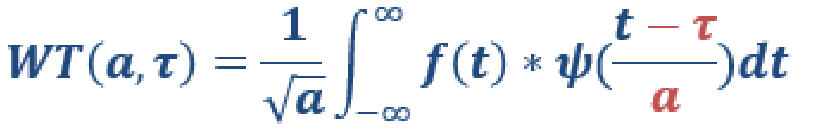
\includegraphics[width=11cm]{little_wave.png}
      \bottomcaption{\xiaowuhao{小波变换函数}}
    \end{figure}
    在该函数中小波变换有两个变量:尺度a(scale)和平移量 $\tau $(translation)。尺度a控制小波函数的伸缩,
    平移量$\tau $控制小波函数的平移。尺度就对应于频率(反比),平移量$\tau$ 就对应于时间。\par
    图像的小波变换是小波应用于图像处理的基础,且基于二维离散小波变换。图像可以看作是二维的矩阵,每次小波变换后,
    图像便分解为4个大小为原来尺寸1/4的子块区域,每一个子块区域包含了相应频带的小波系数,
    相当于在水平方向和坚直方向上进行隔点采样。进行下一层小波变换时,变换数据集中在LL频带上。
    小波系数的空间分布同原始图像的空间分布具有很好的对应关系:\par
    1.LL频带是图像内容的缩略图,它是图像数据能量集中的频带。\par
    2.HL频带存放的是图像水平方向的高频信息,它反映了图像水平方向上的变化信息和边缘信息。\par
    3.LH频带存放的是图像竖直方向的高频信息,它反映了图像在竖直方向上的灰度变化信息和图像边缘信息。\par
    4.HH频带存放的是图像在对角线方向的高频信息,它反映了水平方向和竖直方向上图像灰度的综合变化信息,同时包含了少量的边缘信息。\par
    所以对图像进行一级小波分解和二级小波分解得到的图像的系数分布如下图所示
    \begin{figure}[H]
      \begin{minipage}[t]{0.45\linewidth}
          \centering
          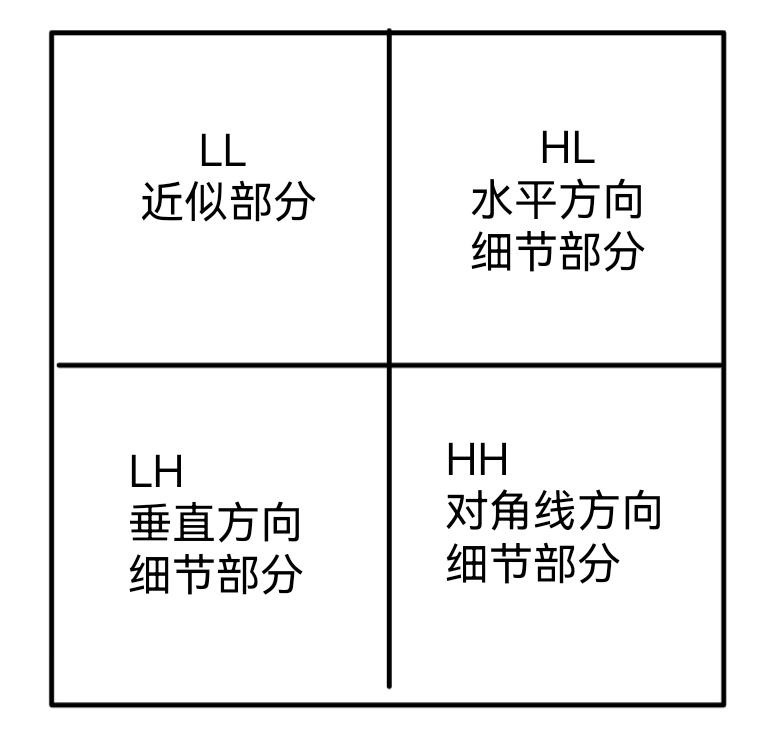
\includegraphics[width=5.5cm,height=5.5cm]{little_wave_1.jpg}
          \caption{一级小波变换系数分布}
      \end{minipage}
      \begin{minipage}[t]{0.45\linewidth}        %图片占用一行宽度的45%
          \hspace{10pt}
          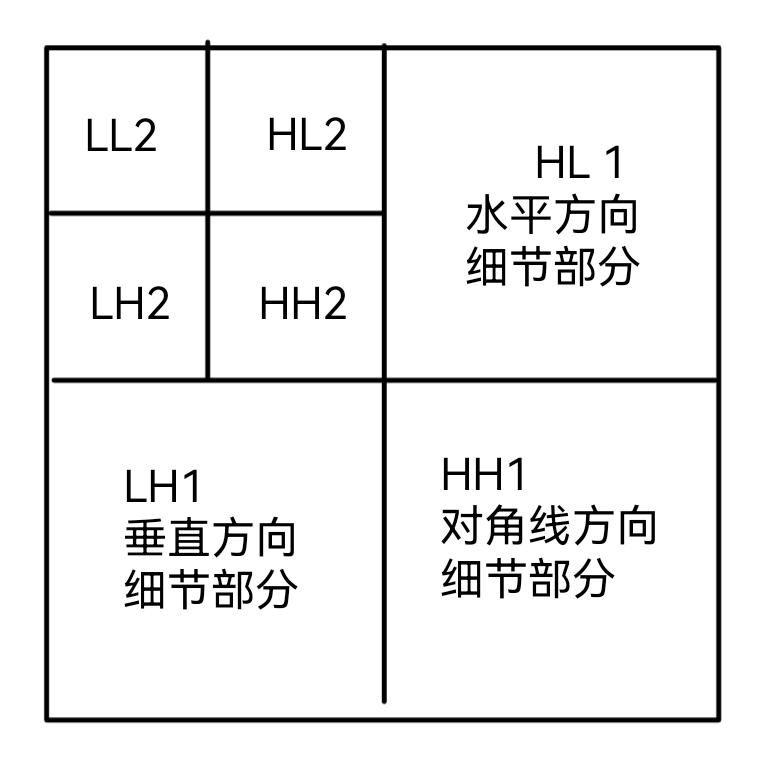
\includegraphics[width=5.5cm,height=5.5cm]{little_wave_2.jpg}
          \caption{二级小波变换系数分布}
      \end{minipage}
    \end{figure}
  \subsection{数据归一化}
    数据的归一化一般是将数据映射到指定的范围,用于去除不同维度数据的量纲以及量纲单位。
    常见的映射范围有$\left [ 0,1 \right ]$  和 $\left [ -1,1 \right ]$ 。\par
    本次实验中采用的归一化方法就是 Min-Max 归一化。也称为离差标准化,是对原始数据的线性变换,
    使结果值映射到$\left [ 0,1 \right ]$之间。转换函数为$x{new}=\frac{x-x{min}}{x{max}-x{min}} $\par
    其中max为样本数据的最大值,min为样本数据的最小值。这种归一化方法比较适用在数值比较集中的情况。
    但是,如果max和min不稳定,很容易使得归一化结果不稳定,使得后续使用效果也不稳定,实际使用中可以用经验常量值来替代max和min。
    而且当有新数据加入时,可能导致max和min的变化,需要重新定义。

  \subsection{奇异值分解生成水印模板}
    对于任意M*N矩阵A,都可以写成$A=U\times \sum \times V^{T} $,其中U和V分别是M*M和N*N的正交矩阵,Σ是M*N的对角矩阵,
    这种变换成为矩阵SVD变换,U和V中分别称作A的奇异向量,Σ是A的奇异值。\par
    在本次实验中对图像做小波分解得到其低频系数LL,然后对LL做单值分解$LL=U\sum V^{T} $,用伪随机序列生成两个正交矩阵
    然后用生成的两个正交矩阵的后d列替换掉U和V的后d列,得到$\widetilde{U}$ 和$\widetilde{V}$\par
    然后用伪随机数生成器生成一个对角矩阵后乘上alpha(强度因子)得到新的对角矩阵$\widetilde{ \sum}$\par
    最后能够得到水印模板watermark=$\widetilde{U}\times \widetilde{ \sum}\times \widetilde{V}$\par
    算法的流程如下图所示
    \begin{figure}[H]
      \centering
      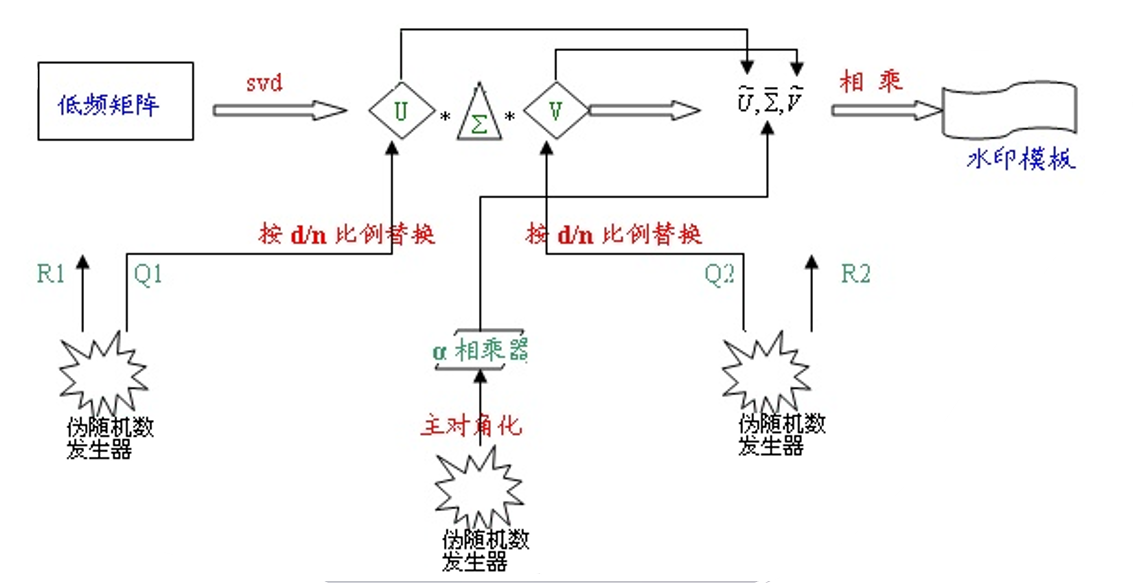
\includegraphics[width=11cm]{SVD_yuanli.png}
      \bottomcaption{\xiaowuhao{SVD生成水印模板流程}}
    \end{figure}
  \subsection{数字水印检测}
    利用原始图像生成一个理论上存在的水印模板(原始水印),从待检测图像中提取可能存在的水印模板(待测水印),计算两者的相关性。
    当两者高度相关时,待测图像含有水印;反之检测不出水印。\par
    原始水印可以通过首先提取出原图的小波低频系数A,然后再提取出将原图进行嵌入水印后提取加有水印的图像的小波系数B
    通过计算可得原始水印为=A-B,然后提取待检测图像的低频小波系数C,计算待测水印=C-B,即可得到原始水印和待测水印。\par
    在比较两个水印的相关性时有两种方法:
    1.常规检测直接相关性值。借助公式$d=\frac{\left | \sum_{i=1}^{M} \sum_{j=1}^{N}W{ij}V{ij}    \right | }{\sqrt{ \sum_{i=1}^{M} \sum_{j=1}^{N}W{ij}V{ij}}*\sqrt{ \sum_{i=1}^{M} \sum_{j=1}^{N}W{ij}V{ij}}  } $
    可以求出原始水印和待测水印的相关性的值,在该公式中,W和V代表两个水印的矩阵,M和N分别代表其大小。\par
    若两个水印的相关性越强,则得到的d越趋近于1,反之则越小\par
    2.DCT域相关性值,首先将原始水印和待测水印进行DCT域的变换后得到的两个矩阵同样利用上述公式计算d的值,得到的d的值越趋近于1则两个水印的相关性越强。
    算法的流程如下图所示
    \begin{figure}[H]
      \centering
      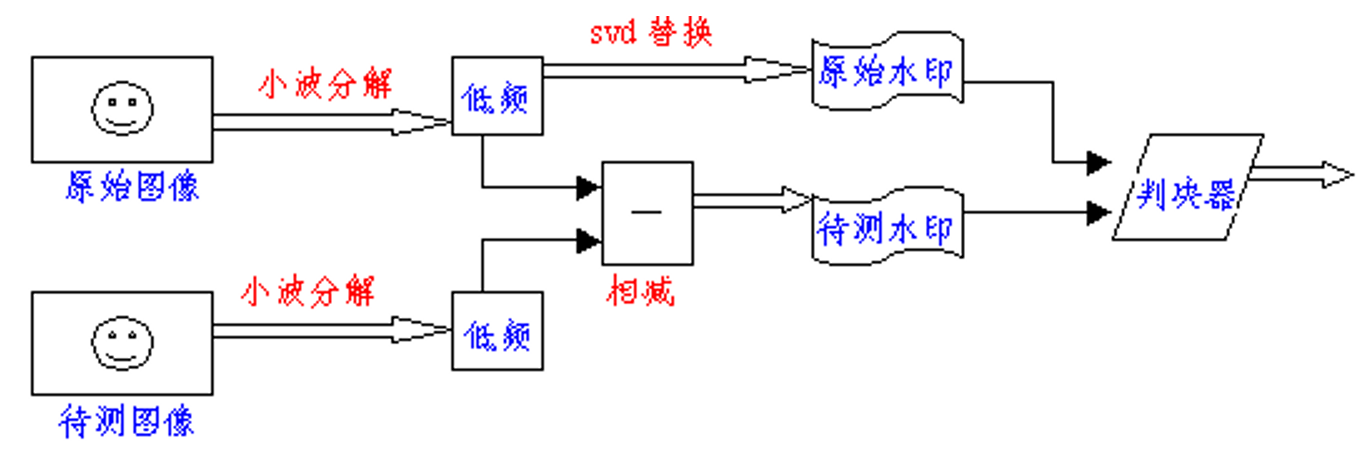
\includegraphics[width=11cm]{W_SVD_find_yuanli.png}
      \bottomcaption{\xiaowuhao{W-SVD水印检测原理}}
    \end{figure}

\section{实验内容:}
\subsection{W-SVD水印生成及嵌入}
    实现对于输入的图像进行W-SVD嵌入水印操作的代码如下所示
    \lstinputlisting[caption={W-SVD水印生成及嵌入},captionpos=b]{E:/matlab_codes/lab_3/W_SVD/W_SVD_hide.m}
\newpage
\subsection{W-SVD水印的检测}
    实现对于待检测图像的水印检测操作的代码如下所示
    \lstinputlisting[caption={W-SVD水印检测},captionpos=b]{E:/matlab_codes/lab_3/W_SVD/W_SVD_find.m}
    该函数调用了获取原图加水印后的低频小波系数的函数W\_SVD\_get\_waterCA代码如下所示
    \lstinputlisting[caption={获取原图加水印后的低频小波系数},captionpos=b]{E:/matlab_codes/lab_3/W_SVD/W_SVD_get_waterCA.m}
\newpage
\subsection{SC图绘制}
    实现在W-SVD水印检测过程中绘制SC图的代码如下所示
    \lstinputlisting[caption={绘制每个参数的SC图},captionpos=b]{E:/matlab_codes/lab_3/W_SVD/output_disp.m}
    该函数调用了绘制单个SC图的函数的代码如下所示
    \lstinputlisting[caption={绘制单个SC图},captionpos=b]{E:/matlab_codes/lab_3/W_SVD/disp_xy.m}
\newpage
\subsection{stirmark工具攻击评价算法鲁棒性}
    实现自动检测攻击后生成的待检测图片的代码如下图所示
    \lstinputlisting[caption={绘制每个参数的SC图},captionpos=b]{E:/matlab_codes/lab_3/W_SVD/attack.m}

\section{实验环境:}
  1.win11操作系统\par
  2.MATLAB R2022a\par
  3.Visual Studio Code 1.84.2 (user setup)\par
  4.Texlive


\section{实验步骤:}
  \subsection{W-SVD水印生成及嵌入}
    \subsubsection{原图小波分解}
      在本次实验中使用的原图为png格式的图片,取出其R色域的信息进行水印的嵌入,首先将水印载体进行一次小波分解
      得到参数C代表各层分解系数和S\_real代表未补足的各层分解系数长度。
    \subsubsection{图像补足}
      为了使后期的实验更加方便,需要将载体转变为正方形的图像即选取载体矩阵行数列数中的较大值作为新的载体矩阵的
      边长,然后将旧载体矩阵赋值到新矩阵中,余下的位置补0。
    \subsubsection{小波分解获取低频系数}
      将补足为正方形的载体矩阵再次进行小波分解,得到参数C代表各层分解系数和S代表各层分解系数长度,然后将得到的两个参数
      传递到函数appcoef2中提取小波分解后的N级低频成分\par
      在得到图像的小波低频系数后需要对数据进行归一化处理,将其映射到区间$\left [ 0,1 \right ]$中,
      最后得到经过处理的小波分解低频系数保存在变量CA中。
    \subsubsection{按照小波低频系数生成水印模板}
      首先将得到的小波低频系数进行SVD变换,分解得到两个正交矩阵U,V和一个对角矩阵Σ,
      然后使用事先设定好种子的随机数生成器生成两个随机正交矩阵,利用随机矩阵的后一定比例的列的值替换掉
      SVD变换两个正交矩阵的后一定比例的列,其中一定比例在本次实验中使用变量radio保存,由此即可得到两个新的正交矩阵
      $\widetilde{U}$ 和$\widetilde{V}$\par
      然后利用设定好种子的随机数发生器生成一个对角矩阵并且零对角矩阵乘强度因子alpha,得到一个新的对角矩阵$\widetilde{ \sum}$
      然后将得到的两个正交矩阵与对角矩阵相乘便能够得到水印模板保存到变量watermark中。
    \subsubsection{获取带有水印的小波低频系数}
      在得到水印模板后将其与先前得到的原图像的小波低频系数直接相加然后将过辐的系数即超过1的系数置为1,将负系数置为0。\par
      由于在小波分解后将低频系数进行了归一化处理,所以在此应当逆用公式将其还原得到加有水印的低频系数保存到变量waterCA中\par
      因为在图像处理时对图像进行了补足处理,在得到的waterCA中会存在有冗余信息,所以需要只保存其原始信息部分。
      图像在补全前进行过一次小波变换操作得到了参数S\_real,该参数的第一行保存着原始图像小波变换后被分解的行数和列数,
      因此只保留waterCA的$1:S\_real(1,1),1:S\_real(1,1)$部分即可,得到的数据保存到变量CA\_tilde中。
    \subsubsection{获得嵌入水印后的图像}
      在得嵌入有水印的低频系数后首先将其转变为只有一行的格式,然后用其代替小波变换得到的C与得到的S进行逆小波变换还原图像的格式。\par
      由于在图像处理之初对图像进行了补全操作,所以在此要裁剪掉补全的部分。\par
      最后再将经过处理得到的图像与G,B两个色域进行融合操作即可得到嵌入水印后的图像。

  \subsection{W-SVD水印的检测}
    \subsubsection{计算原始水印和待测水印}
      在进行相关度分析前首先要对原图进行嵌入水印操作,得到原图嵌入水印后的小波低频系数记为waterCA\_origin,
      然后得到原图的小波低频系数记为CA\_origin然后提取出待检测图像的小波低频系数记为CA\_test\par
      计算得到原始水印watermark\_origin为waterCA\_origin - CA\_origin,\\
      待测水印watermark\_test为CA\_test - CA\_origin
    \subsubsection{计算原始水印和待测水印的相关性}
      首先利用计算相关性的公式计算出常规检测直接相关性值保存到变量\\corr\_coef中\par
      然后将两个水印分别进行DCT变换后取32*32的块利用公式进行相关性的计算将计算的结果保存在变量corr\_DCTcoef中
    \subsubsection{绘制检测结果SC图}
      对小波变换的每一个参数,wavelet(小波函数)、N(小波分解层数)、ratio(替换正交矩阵的比例)、seed(种子)、
      alpha(强度因子)选取一定的范围作为检测的区间,每一次循环遍历单个参数的所有区间调用计算相关性的函数,
      得到该参数的多个取值下的相关性的不同,将其结果进行绘制。对每个参数进行一次上述操作即可得到有关所有参数的SC图。
  \subsection{分析水印算法鲁棒性}
    \subsubsection{嵌入水印后的图像使用stirmark工具生成攻击后的图像}
      修改stirmark工具的配置文件,对已经利用W-SVD嵌入水印的图片进行 \\
      AddNoise、JPEG、MedianCut三种攻击方式得到攻击后的图像,
      然后在output文件夹中对不同攻击方式的图片进行分类整理,以便于之后水印的检测。
    \subsubsection{初始化程序运行参数}
      首先初始化每种攻击方式的参数,将其保存到各自的number数组中,然后定义当前攻击方式n,并且利用变量numbers表示当前攻击方式
      的参数数组,然后根据工具方式拼接出攻击方式所在的文件夹路径,然后读取选定的文件夹路径下攻击方式的所有图片
    \subsubsection{水印检测与绘制结果图}
      对于读取得到的每一个图片都进行一次水印检测操作,将得到的两个相关性分别保存到数组corrs和corr\_DCTs中。
      最后使用corrs和corr\_DCTs绘制当前攻击方式下的相关性折线图。

\section{实验结果与分析:}
  \subsection{W-SVD水印嵌入}
    \begin{itemize}
      \item 运行W-SVD水印嵌入函数得到的结果如下图所示
        \begin{figure}[H]
          \centering
          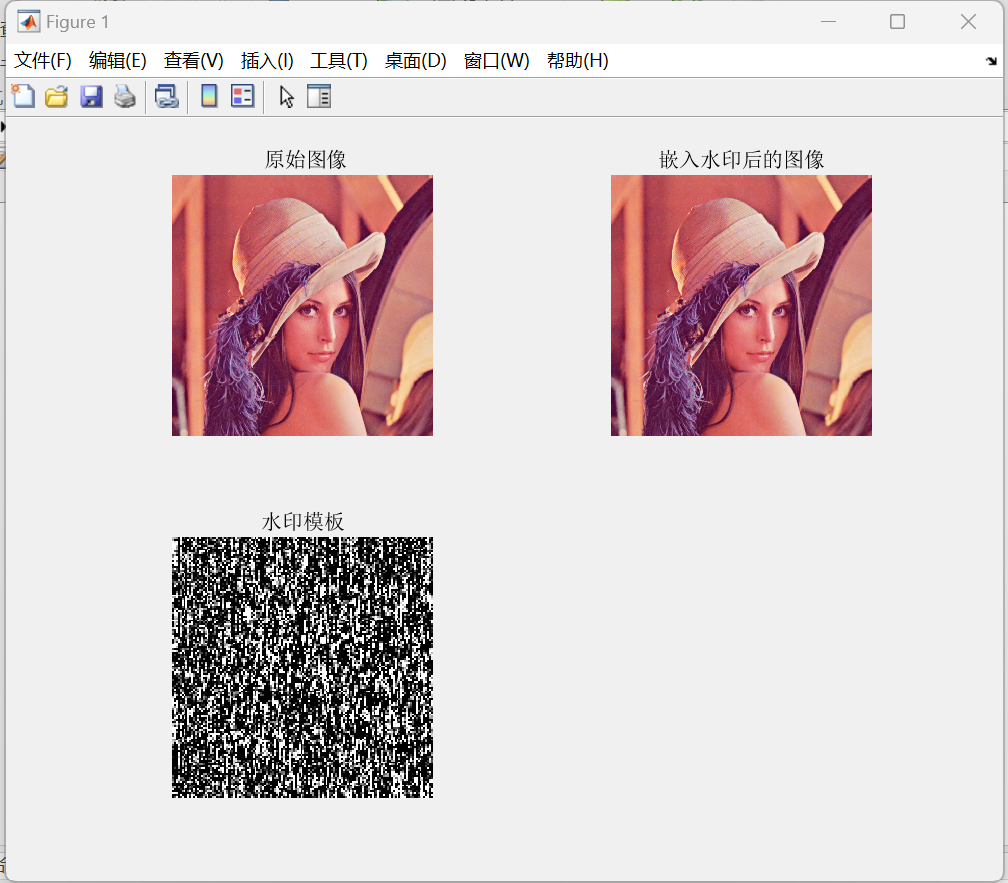
\includegraphics[width=11cm]{W-SVD_hide.png}
          \bottomcaption{\xiaowuhao{W-SVD水印嵌入结果}}
        \end{figure}
        该函数运行后能够显示出进行W-SVD水印嵌入前后的图像还能够得到嵌入的水印模板的图像
    \end{itemize}
\newpage
  \subsection{W-SVD水印检测}
    \begin{itemize}
      \item 检测在W-SVD水印嵌入过程中,种子值的不同对水印相关性的影响如下图所示
        \begin{figure}[H]
          \centering
          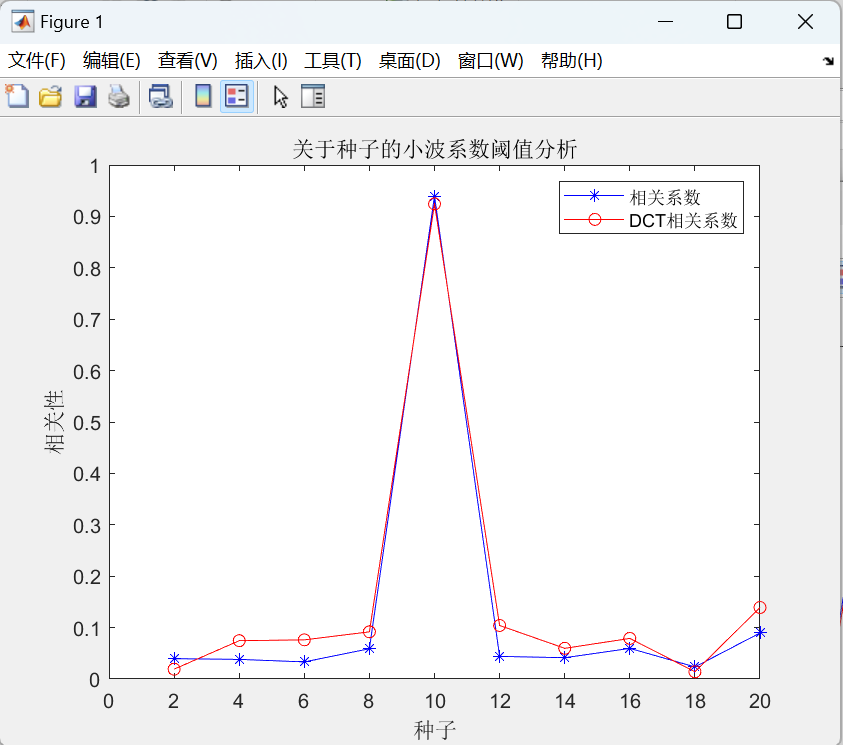
\includegraphics[width=9cm]{W-SVD_find_seed.png}
          \bottomcaption{\xiaowuhao{种子值-相关性关系}}
        \end{figure}
      \item 检测在W-SVD水印嵌入过程中,小波变换次数的不同对水印相关性的影响如下图所示
        \begin{figure}[H]
          \centering
          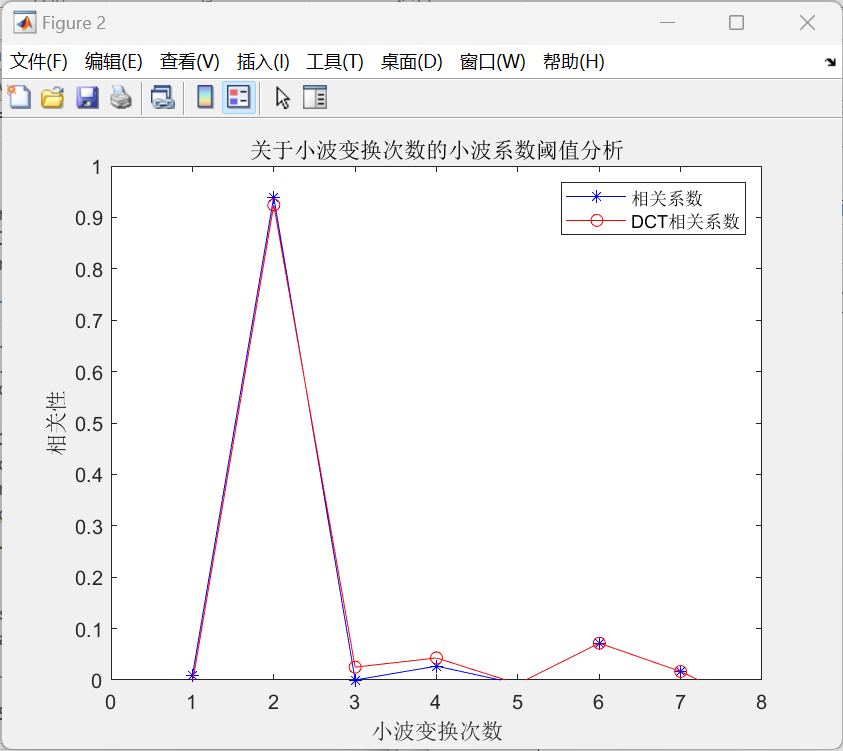
\includegraphics[width=9cm]{W-SVD_find_N.png}
          \bottomcaption{\xiaowuhao{小波变换次数-相关性关系}}
        \end{figure}
      \item 检测在W-SVD水印嵌入过程中,替换比例的不同对水印相关性的影响如下图所示
        \begin{figure}[H]
          \centering
          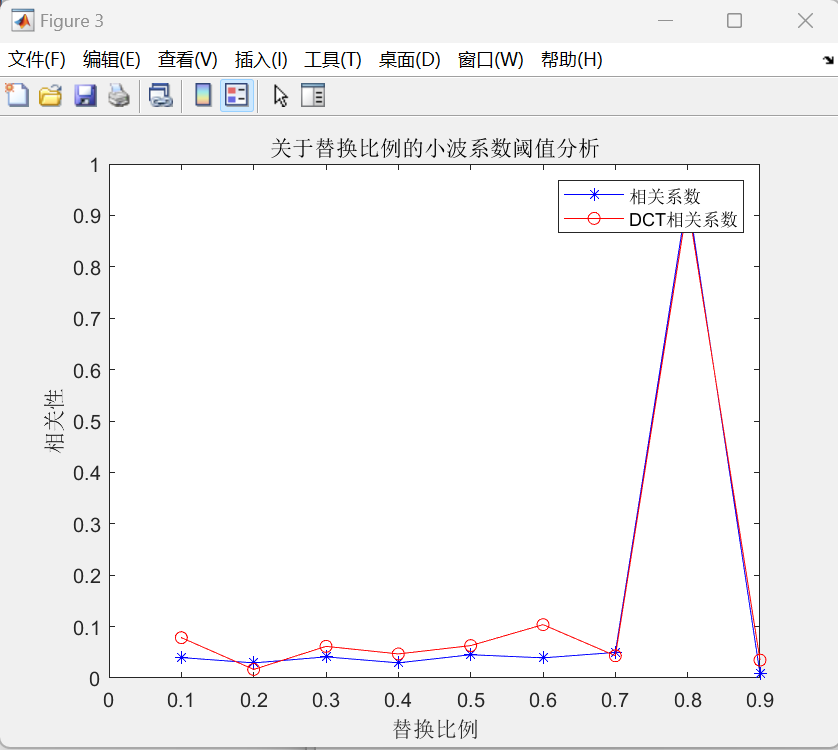
\includegraphics[width=9cm]{W-SVD_find_ratio.png}
          \bottomcaption{\xiaowuhao{替换比例-相关性关系}}
        \end{figure}
      \item 检测在W-SVD水印嵌入过程中,小波函数种类的不同对水印相关性的影响如下图所示
        \begin{figure}[H]
          \centering
          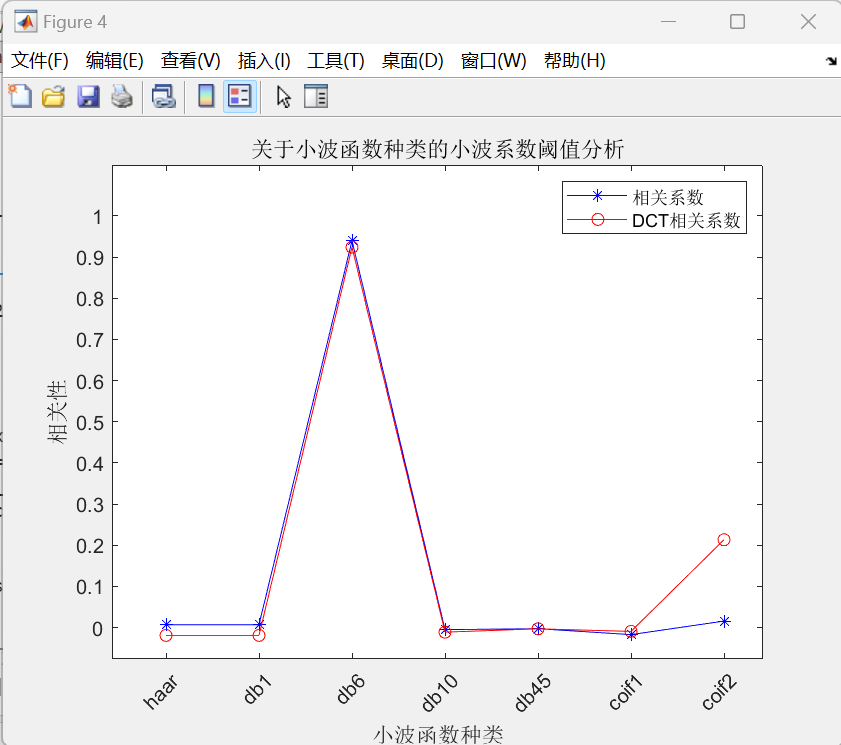
\includegraphics[width=9cm]{W-SVD_find_wavelet.png}
          \bottomcaption{\xiaowuhao{小波函数种类-相关性关系}}
        \end{figure}
\newpage
      \item 检测在W-SVD水印嵌入过程中,强度因子的不同对水印相关性的影响如下图所示
        \begin{figure}[H]
          \centering
          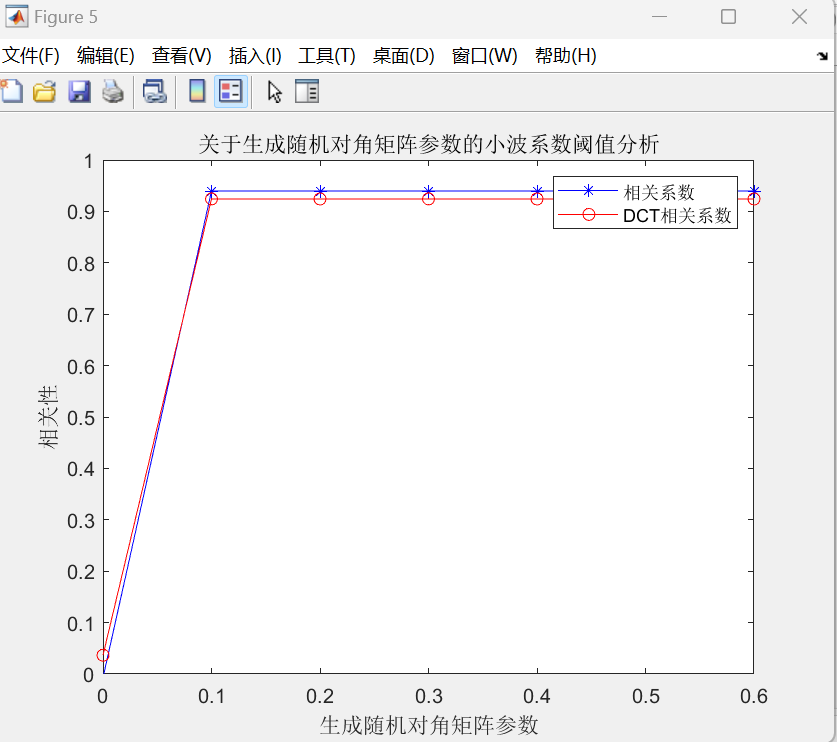
\includegraphics[width=9cm]{W-SVD_find_alpha.png}
          \bottomcaption{\xiaowuhao{强度因子-相关性关系}}
        \end{figure}
    \end{itemize}
  \subsection{分析水印算法鲁棒性}
    \begin{itemize}
      \item 加噪处理NOISE\par
        加噪后的图像如下图所示
        \begin{figure}[H]
          \centering
          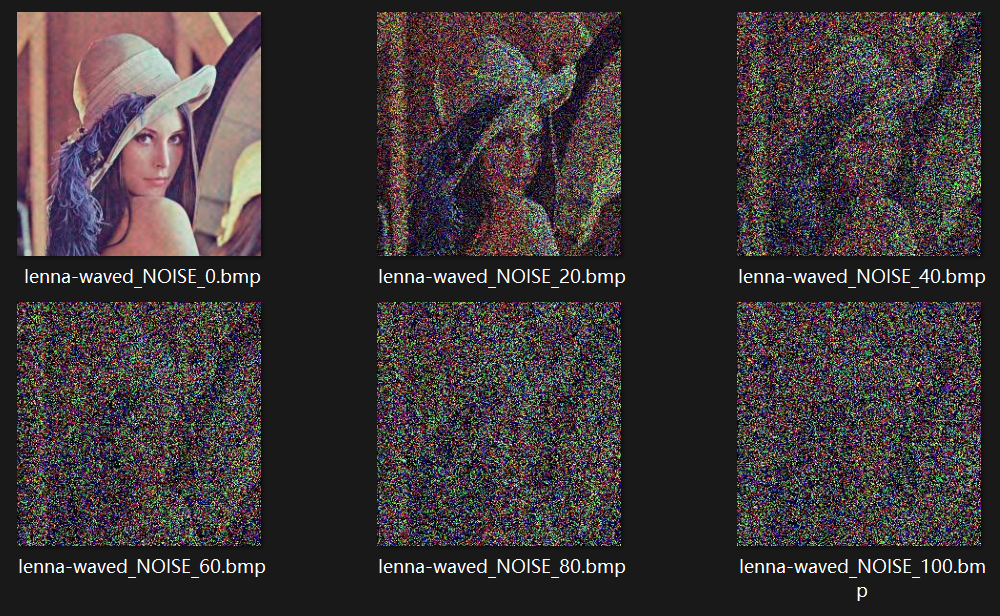
\includegraphics[width=11cm]{imgs_noise.png}
          \bottomcaption{\xiaowuhao{加噪处理后的图像}}
        \end{figure}
\newpage
        将使用不同参数的加噪处理后的图像进行水印检测后得到的结果如下图所示
        \begin{figure}[H]
          \centering
          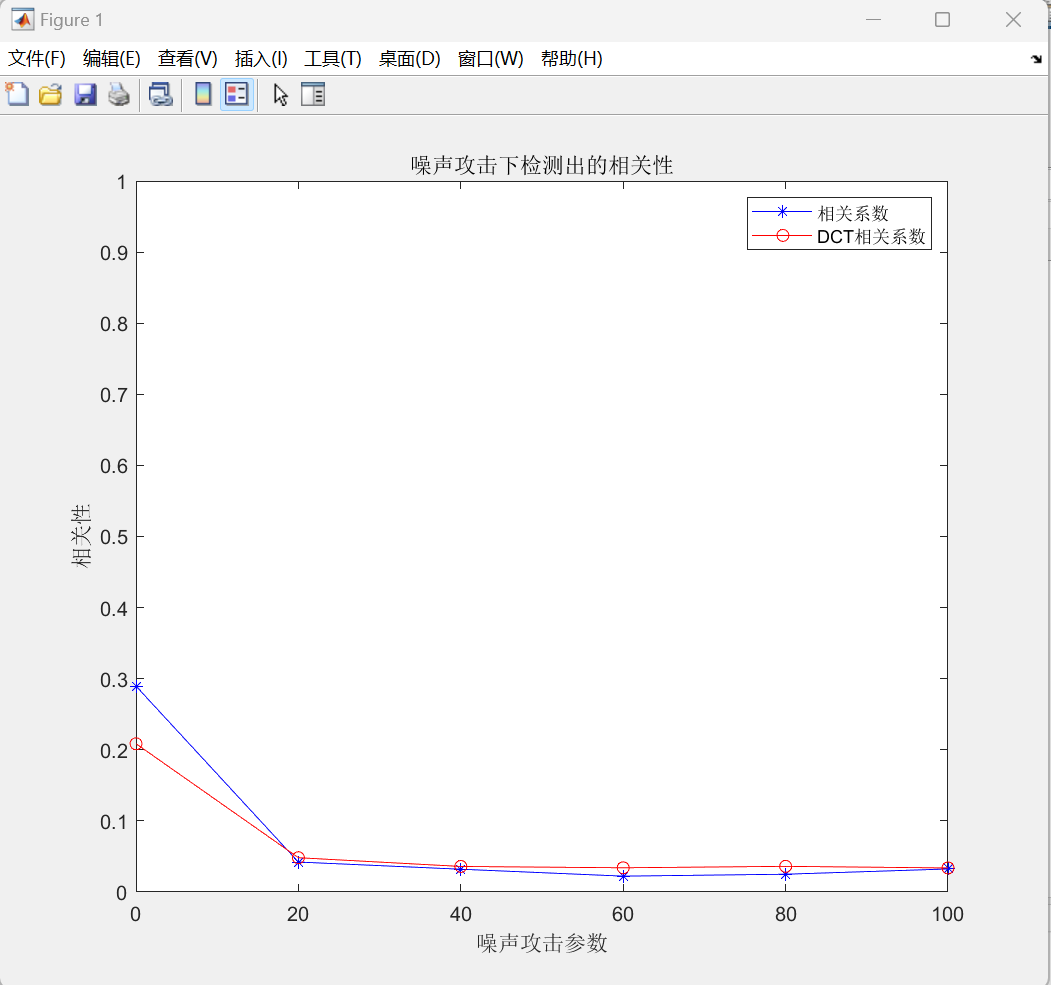
\includegraphics[width=11cm]{attack_noise.png}
          \bottomcaption{\xiaowuhao{加噪处理后的相关性}}
        \end{figure}
        
        通过分析相关性的折线图可以看出在加噪信号为0的情况下,待检测的图片尚且保存有较高的相关性,能够检测出有
        水印的嵌入,且直接计算出的相关性高于在DCT域计算出的相关性,但在有加噪信号的条件下待检测图片的相关性就骤降至0.1以下,
        不能够有效的分析出是否有水印的嵌入。且两个计算相关性的方法无较大差别\par
        由此可以断定,W-SVD水印嵌入算法在面对加噪处理时鲁棒性较低。
\newpage
      \item JPEG攻击\par
        JPEG压缩处理后的图像如下图所示
        \begin{figure}[H]
          \centering
          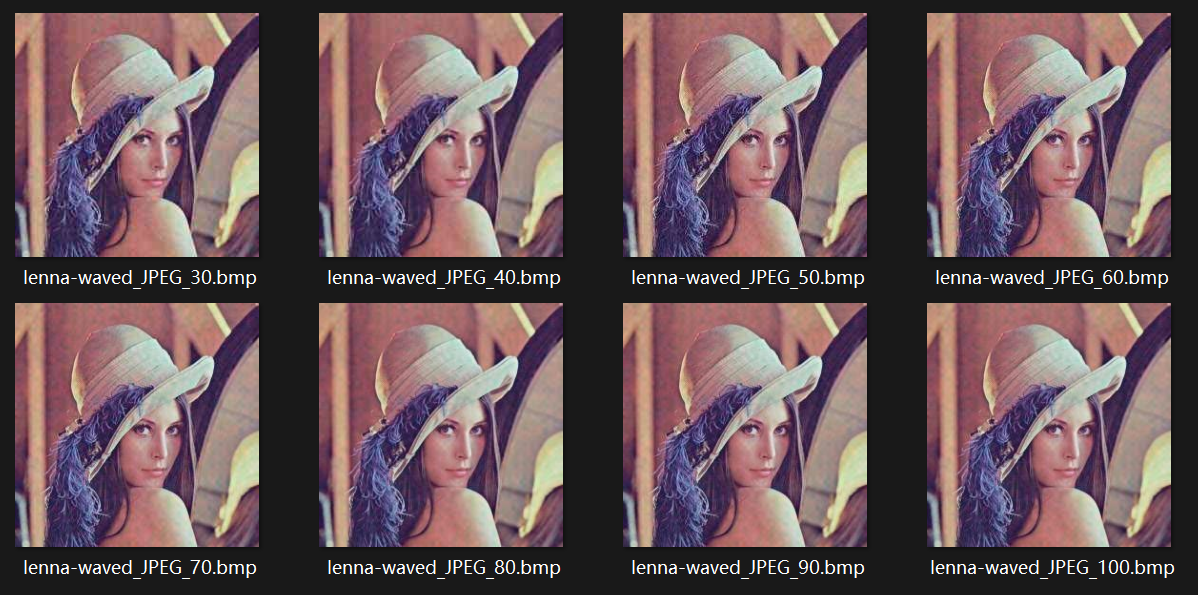
\includegraphics[width=11cm]{imgs_jpeg.png}
          \bottomcaption{\xiaowuhao{JPEG压缩处理后的图像}}
        \end{figure}
        将使用不同参数的JEPG压缩处理后的图像进行水印检测后得到的结果如下图所示
        \begin{figure}[H]
          \centering
          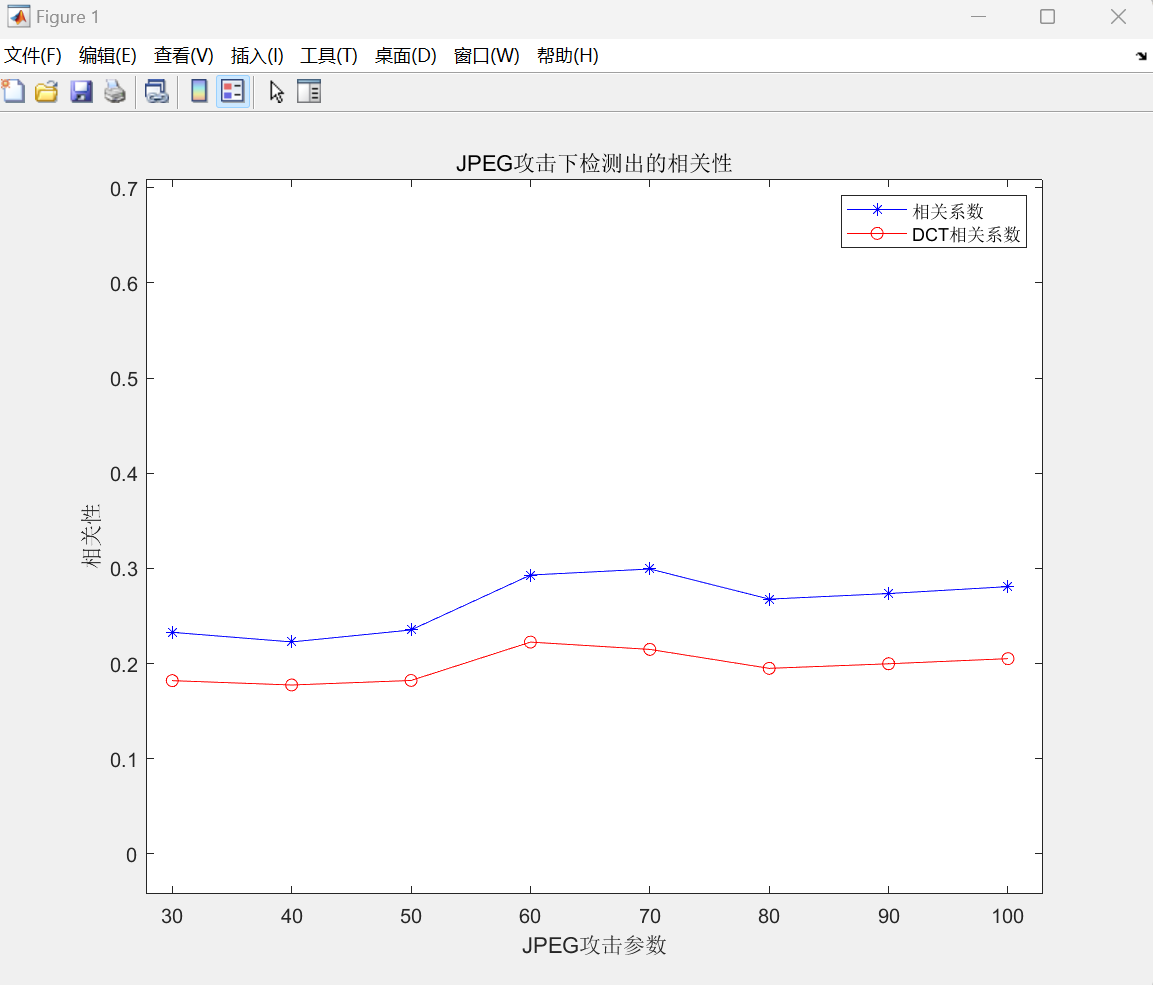
\includegraphics[width=11cm]{attack_jpeg.png}
          \bottomcaption{\xiaowuhao{JPEG压缩处理后的相关性}}
        \end{figure}
        通过分析相关性的折线图可以看出在JPEG压缩率在30-50时,图像的相关性维持在0.2左右,仍然有一定的识别能力
        而且当压缩率到达60-70时,图像的相关性会保持在0.3左右,相比于压缩率较低的情况水印的识别能力更强。
        当压缩率到达80-100时,图像的相关性会降低到0.25左右,相比于压缩率中等的情况,识别能力较差。且直接计算的相关性
        始终高于在DCT域计算出来的相关性\par
        由此可以断定,W-SVD水印嵌入算法在面对JPEG压缩处理时的鲁棒性较高,相关性仍能够维持在一定的水平,
        但是压缩率在60-70时相比于更高或更低的压缩率,其相关性更高,因此在采取JPEG对嵌入水印的图像进行攻击时应当
        选取较低或者较高的压缩率,不能选择压缩率在60-70之间进行压缩。

      \item 中值滤波MEDIAN\par
        中值滤波处理后的图像如下图所示
        \begin{figure}[H]
          \centering
          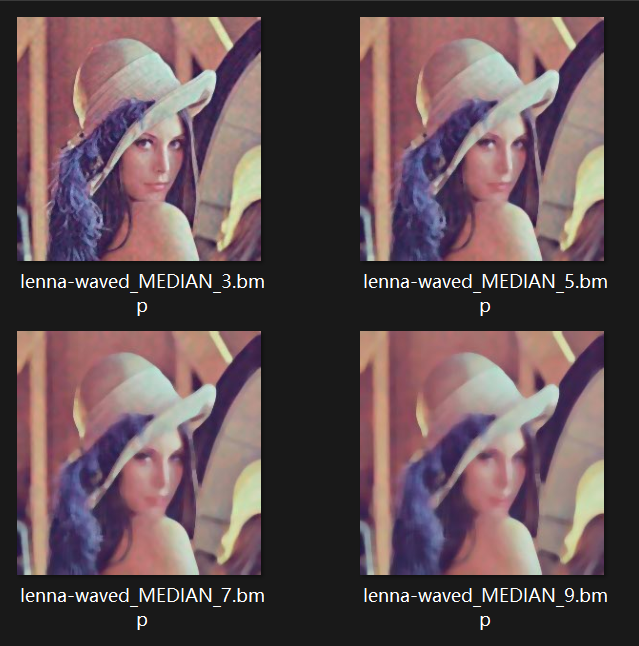
\includegraphics[width=11cm]{imgs_median.png}
          \bottomcaption{\xiaowuhao{中值滤波处理后的图像}}
        \end{figure}
\newpage
        将使用不同参数的中值滤波处理后的图像进行水印检测后得到的结果如下图所示
        \begin{figure}[H]
          \centering
          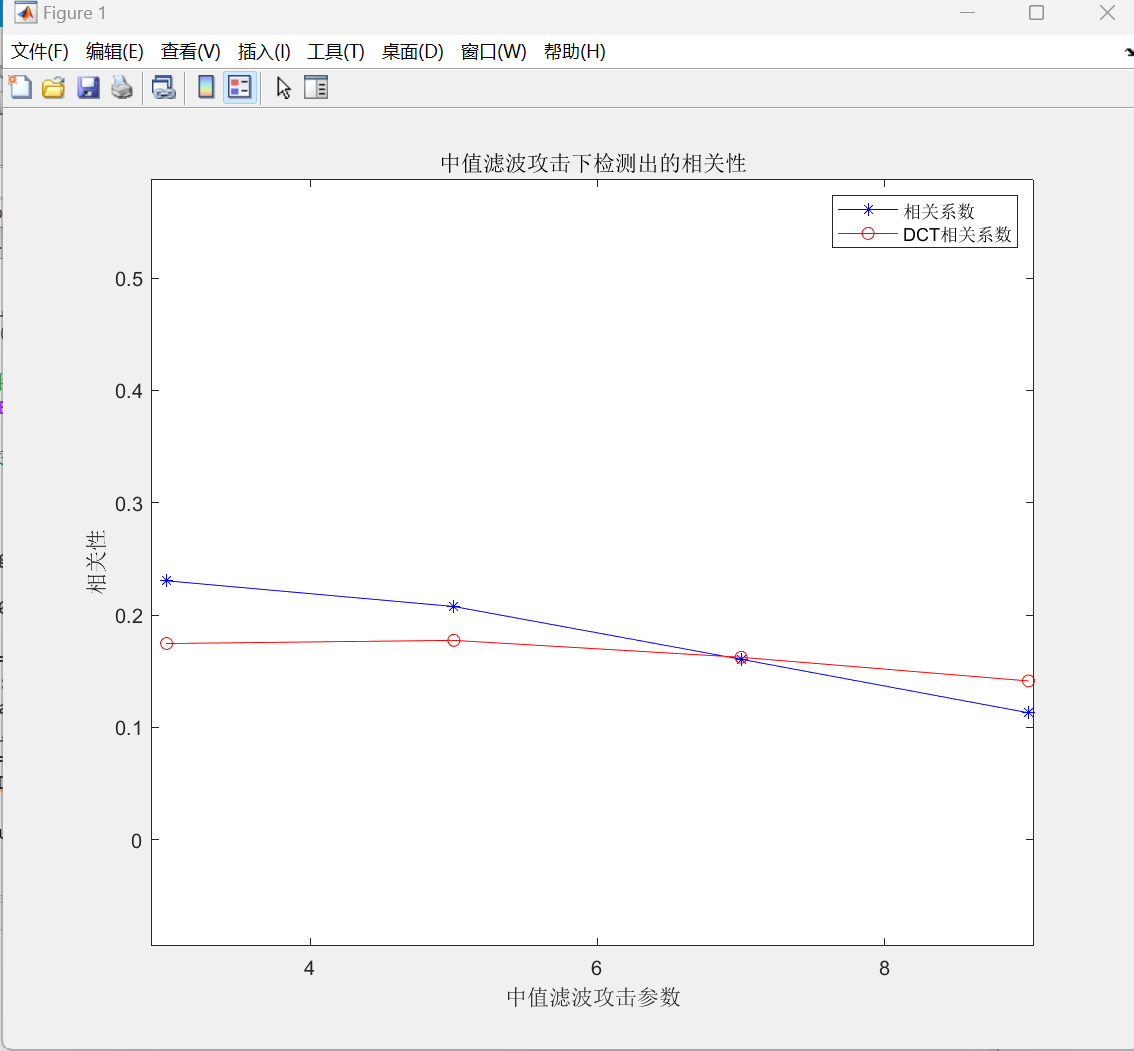
\includegraphics[width=9cm]{attack_median.png}
          \bottomcaption{\xiaowuhao{中值滤波MEDIAN处理后的相关性}}
        \end{figure}
        通过分析折线图可以得出随着滤波参数核的变大,待检测图像的相关性在缓慢降低。在核为7之前,DCT检测的能力较弱,
        检测到的相关性相比于直接计算较低。而在核大于7的情况下则DCT的检测能力较强,检测到的相关性相比于直接计算要高\par
        由此可以断定,W-SVD水印嵌入算法在面对中值滤波时保持有一定的鲁棒性,且随着中值滤波核的增大,其水印被检测的能力越低。
        因此在选用中值滤波对W-SVD水印嵌入算法进行攻击时,应当尽量选用较大的核。

      \item 总结\par
        分析三种不同的攻击方式攻击后图片的检测结果可以看出,W-SVD水印嵌入算法在面对加噪处理时的鲁棒性最低,且近乎无法检测出
        是否嵌入水印,但是使用该方法对原图的损害较大。W-SVD水印嵌入算法在面对JPEG压缩处理时的鲁棒性最高,能够检测的程度始终
        维持在一定的水平,并且该种方法对原图的损害较小。W-SVD水印嵌入算法在面对中值滤波时保持有一定的鲁棒性,
        但是使用该方法对原图的损害较大。
    \end{itemize}
  \subsection{分析不同算法参数情况对水印性能的影响}
    \subsubsection{水印性能衡量标准}
      在本次实验中首先将原图嵌入水印后传入stirmark中进行median攻击,选取使用核为3的攻击后的图像进行检测
      通过比较相关性来衡量当前参数对水印性能的影响。
    \subsubsection{小波分解层数N}
      \begin{table}[H]
        \caption{小波分解层数不同对水印性能的影响}\label{tab1}
          \centering
        \begin{tabular*}{0.75\textwidth}{@{\extracolsep{\fill}}lcc}
            \toprule
            小波分解层数           &直接相关性        &DCT域相关性                         \\
            \midrule
            1                     &0.0615           &0.0892                                      \\
            2                     &0.2305           &0.1747                                      \\
            3                     &0.3131           &0.2607                                        \\
            4                     &0.1270           &0.1270                                    \\ 
            5                     &0.1684           &0.1684\\
            \bottomrule
        \end{tabular*}
      \end{table}
      观察小波分解层数的不同得出的结果可以看出,当小波分解的层数是3层时,该水印的鲁棒性达到峰值,且当小波分解
      层数为1层时该水印的鲁棒性最弱,在攻击后不能够被检测。由此可见小波分解的层数对水印的鲁棒性有较大影响
      
    \subsubsection{小波函数种类wavelet}
      \begin{table}[H]
        \caption{小波函数种类不同对水印性能的影响}\label{tab2}
          \centering
        \begin{tabular*}{0.75\textwidth}{@{\extracolsep{\fill}}lcc}
            \toprule
            小波函数种类           &直接相关性        &DCT域相关性                         \\
            \midrule
            haar                     &0.3445           &0.3445                                      \\
            db1                      &0.3445           &0.3445                                      \\
            db6                      &0.3132           &0.2608                                        \\
            db10                     &0.2130           &0.1833                                    \\ 
            coif1                    &0.3422           &0.3188\\
            \bottomrule
        \end{tabular*}
      \end{table}
      观察小波分解种类的不同得出的结果可以看出,当小波分解函数为haar、db1、coif1、db6时,该水印的鲁棒性没有较大差别,
      均维持在0.3左右,但是小波分解函数为db10时,该水印的鲁棒性较低,只维持在0.2左右。由此可见小波分解的函数种类对
      水印的鲁棒性影响较小

    \subsubsection{强度因子alpha}
      \begin{table}[H]
        \caption{强度因子不同对水印性能的影响}\label{tab3}
          \centering
        \begin{tabular*}{0.75\textwidth}{@{\extracolsep{\fill}}lcc}
            \toprule
            强度因子                 &直接相关性        &DCT域相关性                         \\
            \midrule
            0                       &-0.5000           &-0.5897                                      \\
            0.1                     &0.0614           &0.0619                                      \\
            0.2                     &0.1417           &0.1239                                        \\
            0.3                     &0.2084           &0.1768                                    \\ 
            0.4                     &0.2639           &0.2192\\
            \bottomrule
        \end{tabular*}
      \end{table}
      观察强度因子的变化得出的结果可以看出,强度因子的值越大,得到的水印的鲁棒性就越强。且强度因子对
      水印的鲁棒性的影响较大。

    \subsubsection{种子值seed}
      \begin{table}[H]
        \caption{种子值不同对水印性能的影响}\label{tab4}
          \centering
        \begin{tabular*}{0.75\textwidth}{@{\extracolsep{\fill}}lcc}
            \toprule
            种子值                 &直接相关性        &DCT域相关性                         \\
            \midrule
            2                      &0.2439           &0.1928                                      \\
            5                      &0.2832           &0.2541                                      \\
            10                     &0.2639           &0.2192                                        \\
            20                     &0.3087           &0.2601                                    \\ 
            30                     &0.2752           &0.2276\\
            \bottomrule
        \end{tabular*}
      \end{table}
      观察种子值的不同的变化结果可以看出,所有的种子值得出的结果均在0.2-0.3之间且彼此的值相差不大。所以
      种子值对水印的鲁棒性的影响较小。

    \subsubsection{替换比例ratio}
      \begin{table}[H]
        \caption{替换比例不同对水印性能的影响}\label{tab5}
          \centering
        \begin{tabular*}{0.75\textwidth}{@{\extracolsep{\fill}}lcc}
            \toprule
            替换比例                 &直接相关性        &DCT域相关性                         \\
            \midrule
            0.6                      &0.4186           &0.4010                                      \\
            0.7                      &0.3580           &0.3484                                      \\
            0.8                      &0.4105           &0.3934                                        \\
            0.9                      &0.3620           &0.3398                                    \\ 
            0.99                     &0.3087           &0.2601\\
            \bottomrule
        \end{tabular*}
      \end{table}
      观察替换比例不同时的结果可以看出,当替换比例为0.6和0.8时,水印的鲁棒性最强,相关性为0.4左右,而当
      替换比例为0.7和0.9时水印的鲁棒性相对变弱,替换比例为0.99时水印的鲁棒性达到最弱。由此可见替换比例
      对水印的鲁棒性的影响较大。

\section{总结及心得体会:}
  1.在本次实验中学习了对于图像使用W-SVD的算法嵌入数字水印以及该种数字水印的检测方法。\par
  2.通过对W-SVD水印嵌入算法的不同方式的攻击得出了W-SVD算法在面对不同的攻击方式的鲁棒性。\par
  3.在本次实验中明白了即使是相同的图像在matlab中以矩阵的方式存储时也会因为其拓展名的不同会造成两个图像矩阵的不同。\par
  4.学习到了在数字水印的嵌入过程中不仅仅要考虑嵌入后能否被检测出来,更要考虑待测图像在面对不同种类的攻击时的鲁棒性。\par
\newpage
\section{《人工智能背景下的数字水印》学习心得}
  \subsection{水印的历史、分类和应用}
    在该部分下讲述了隐写的产生以及水印这一工具的产生背景,然后介绍了数字水印在数字媒体中的广泛应用。
    随后介绍了可逆水印出现的原因以及水印在其他方面的拓展应用,了解到了例如User-Cloud、图像上传、图像取回等
    与数字水印相关的协议,并且了解到数字水印借助其鲁棒性来解决很多安全问题。强调了水印的鲁棒性的重要性。
  \subsection{基于深度学习模型的水印}
    在该部分讲解了如何使用深度学习的大致框架框架END来训练模型。讲解了HiDDeN这一深度学习水印,这一方案虽然能够实现端到端的
    训练并且具有很好的透明性和应对失真鲁棒性但是在面对真实JPEG压缩时的鲁棒性却不强。\par
    借由HiDDeN水印提出的挑战问题提出了MBRS的解决方案,该方案能够有效的提升JPEG压缩的鲁棒性。\par
    介绍了保证嵌入器和提取器之间更好耦合的水印算法De-END,通过在嵌入器之前添加一个提取器,两个提取器共享权重的方式来实现
    两者之间更高质量的耦合\par
    为了保证嵌入器和提取器在参数和结构上完美耦合,提出了可逆网络这一解决思路,在鲁棒性的前提下进一步优化了透明性。\par
    介绍了跨媒介鲁棒水印的概念,这一概念与先前介绍的抗摄屏水印有一定的相关性,这一水印的最大的难点就在于真实的物理过程失真
    非常复杂且不可导,而且相比于数字处理更难建模。针对这一问题的解决方法有模拟拍摄过程的噪声层,利用可导过程模拟真实物理失真来对
    水印模型进行训练。该解决方案有LFM和DeNoL等模型。其他的针对这一问题的解决方法有仅训练提取器的水印方案,介绍了该方案下的
    具体模型DTW。\par
    介绍了文档水印、抗翻录音频水印和3D模型水印的背景和相关工作。
  \subsection{保护深度学习模型的水印}
    该部分介绍了深度学习模型当前所面临的知识产权保护的需求,讲解了解决这一需求的白盒水印和黑盒水印以及深度模型水印
    所面临的各种攻击方式。不仅仅是深度学习模型,图像处理和生成模型同样也需要数字水印的保护。
  \subsection{生成式人工智能鉴别水印}
    该部分首先提出了大语言模型生成文本的危害以及国家对AI生成内容的监督以及其检测方案GPTzero但是该种方法检测准确率不高
    并且受文本内容的影响较大。同样也介绍了基于深度学习的检测方法但是其仍然具有脆弱性且在现实复杂的环境下非常容易被干扰。
    最后提出可以通过生成内容水印、黑盒水印或者白盒水印来抵抗大语言模型生成文本的危害。\par
    介绍了语音克隆技术的产生以及其风险,急需音色水印来对音色权进行保护,但是如果攻击者能够仿造被攻击者的音色的话
    会不会能够将音色水印一同仿造呢?\par
    最后介绍了图像概念水印来防止攻击者训练AI模仿画家的图像风格来保护画家等创作者的权利。但是图像概念水印如何能够让人们信服
    并且解决图像风格归属权的问题呢?
    

\vspace{4cm}
\end{document}
